\chapter*{Capítulo 2 \vspace{0.5cm} \break Desarrollo del nuevo sistema}
\setcounter{chapter}{2}
\setcounter{section}{0}
\addcontentsline{toc}{chapter}{Capítulo 2: Desarrollo del nuevo sistema}

En el siguiente capítulo se presenta la propuesta de solución para la problemática planteada: el nuevo sistema SECPROIT. Para que el desarrollo de un proyecto concluya con éxitos, primero debe realizarse el diseño de lo que se pretende obtener, así como analizar los requisitos que debe cumplir. A lo largo de este capítulo se presentarán los diagramas utilizados en la elaboración del sistema, se explicará como está estructurado y cuáles son sus funciones. Cabe destacar que este nuevo diseño parte del que se tenía anteriormente en el SECPROIT, por lo que se realizarán algunas comparaciones dicho modelo.

\section{Descripción del negocio}
Como ya se ha observado en secciones anteriores, lo que se pretende conseguir con este nuevo sistema es rectificar las limitaciones existentes en el SECPROIT actual. Para ello, el nuevo software debe satisfacer el objetivo principal: capacitar a los operarios ante los procesos productivos de una fábrica.
Partiendo de esa idea, esta solución debe poseer un modelo de entrenamiento que ponga a prueba a los operarios de la industria, además, debe contar con un administrador que sea el responsable de incluir a los todos usuarios.

A la hora de realizar el entrenamiento, se deben evaluar tres etapas fundamentales: una para validar los conocimientos sobre las variables, otra para comprobar las causas por las que la variable representa un peligro y la última donde se analicen las recomendaciones que se pueden seguir en caso de que ocurra una falla provocada por esa causa. Si el trabajador logra superar estas etapas, puede darse por aprobado el entrenamiento de ese proceso.

\subsection{Modelo de dominio}
Un modelo de dominio es la representación de las clases conceptuales del mundo real, no de componentes de software. Su utilidad radica en ser una forma de inspiración para el diseño de entidades. Es el artefacto clave en el análisis orientado a objetos \cite{Herchi2012}.

El modelo de dominio de este sistema (\textsl{Figura \ref{fig:dominio}}) no es muy diferente al modelo origina del sistema SECPROIT. A la hora de representarlo, se tuvieron en cuenta una serie de colores a modo de guía:

\begin{itemize}
\item \textbf{Azul}: representa aquellas entidades que no sufrieron ningún cambio significativo con respecto al sistema anterior
\item \textbf{Amarillo}: representa aquellas entidades que fueron modificadas, pero que siguen cumpliendo las mismas funciones
\item \textbf{Verde}: representa las entidades que son totalmente nuevas, que no existen el sistema anterior
\end{itemize}

\begin{figure}[h]
\centering
 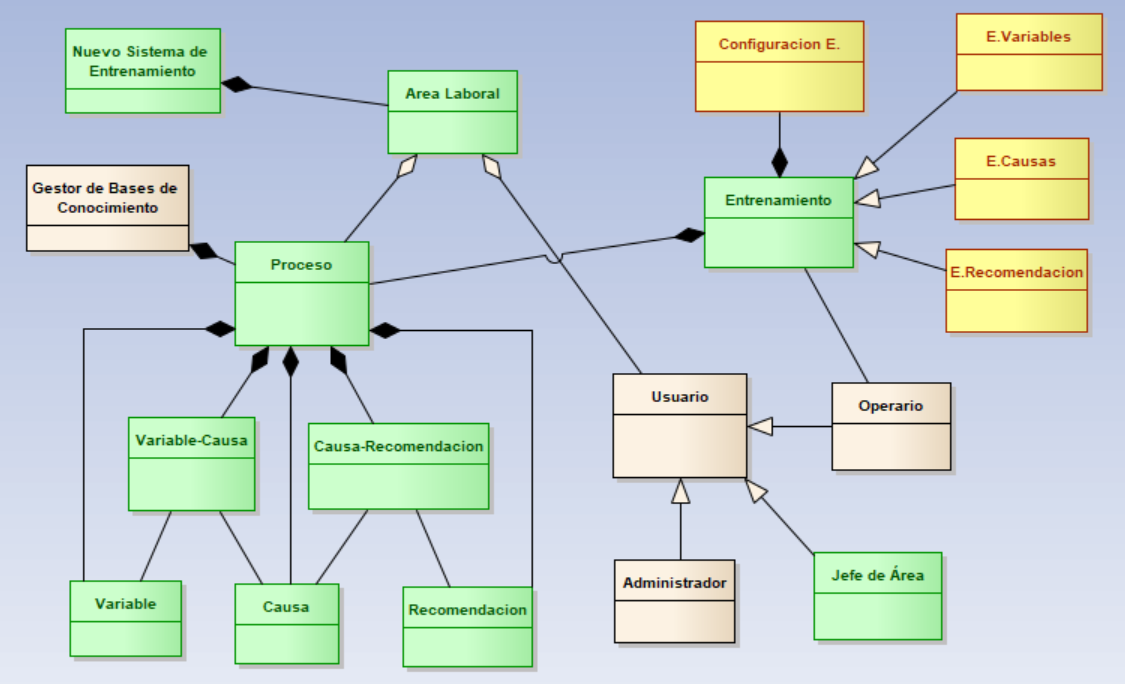
\includegraphics[width=0.7\linewidth]{imagen/dominio.png}
 \caption{Modelo de dominio}
 \label{fig:dominio} 
\end{figure}

La razón por la que algunas entidades (\textsl{Tabla \ref{tab:ent-azul}})  no sufrieron cambios es porque, basados en las tareas que desempeñan, no varían sus funciones con este nuevo modelo. Sin embargo, más adelante pueden presentar modificaciones en algunos aspectos.
Las entidades que cambiaron (\textsl{Tabla \ref{tab:ent-amarilla}}), indican que también se realizaron arreglos en la estructura que estas seguían, es decir, variaciones en la base de datos y en las clases del sistema.
Por último, las entidades nuevas (\textsl{Tabla \ref{tab:ent-verde}}) son clases que fueron agregadas desde cero para rectificar alguna limitación.

\begin{table}[h]
\begin{center}
\begin{tabular}{ | c | p{10cm} | }
\hline
\textbf{Entidad} & \textbf{Descripción} \\
\hline
Área & Representa el lugar donde laboran los trabajadores, posee un identificador y es donde están presentes los procesos \\
\hline
Usuario & Representa a la persona que va interactuar con el sistema \\
\hline
Administrador & Es un tipo de usuario, se encarga de administrar las entidades del sistema (áreas y demás usuarios) \\
\hline
Operario & Es un tipo de usuario, se encarga de realizar los entrenamientos \\
\hline
Base de datos & Representa el archivo \textsf{anm} \\
\hline
Base de reglas & Representa el archivo \textsf{drl} \\
\hline
Drools & Es la entidad que permite ejecutar las reglas del proceso \\
\hline
Variable & Forma parte de la información contenida en la base de datos del proceso, se evalúan en la primera etapa \\
\hline
Causa & Forma parte de la información contenida en la base de datos del proceso, se evalúan en la segunda etapa \\
\hline
Recm. & Forma parte de la información contenida en la base de datos del proceso, representa las recomendaciones y se evalúan en la tercera etapa \\
\hline
Variable-Causa & Forma parte de la información contenida en la base de reglas del proceso, se evalúan en la primera etapa \\
\hline
Causa-Recm. & Forma parte de la información contenida en la base de reglas del proceso, se evalúan en la primera etapa \\
\hline
\end{tabular}
\caption{Modelo de dominio: entidades que no sufrieron cambios}
\label{tab:ent-azul}
\end{center}
\end{table}

\begin{table}[H]
\begin{center}
\begin{tabular}{ | c | p{5cm} |  p{5cm} | }
\hline
\textbf{Entidad} & \textbf{Descripción} & \textbf{Cambios}\\
\hline
Sistema SECPROIT & Representa el sistema & Cambian sus entidades y funciones \\
\hline
Jefe e área & Es un tipo de usuario, administrar los procesos & Antes era especialista y solo creaba los procesos \\
\hline
Proceso & Representa los procesos & Se le agrega un nuevo atributo: la configuración \\
\hline
Entrenamiento & Representa el entrenamiento del usuario & Se le agregan las etapas \\
\hline
\end{tabular}
\caption{Modelo de dominio: entidades que sufrieron cambios}
\label{tab:ent-amarilla}
\end{center}
\end{table}

\begin{table}[t]
\begin{center}
\begin{tabular}{ | c | p{10cm} | }
\hline
\textbf{Entidad} & \textbf{Descripción} \\
\hline
Configuración & Representa la configuración de un proceso, es decir, las características que este posee para generar un entrenamiento \\
\hline
Etapas & Representa las etapas del entrenamiento, existen tres por cada uno \\
\hline
E-Variable & Es un tipo de etapa, donde se evalúan las variables \\
\hline
E-Causa & Es un tipo de etapa, donde se evalúan las causas \\
\hline
E-Recm. & Es un tipo de etapa, donde se evalúan las recomendaciones \\
\hline
\end{tabular}
\caption{Modelo de dominio: entidades nuevas}
\label{tab:ent-verde}
\end{center}
\end{table}

\subsection{Reglas del negocio}
Las reglas de un negocio son directrices y restricciones que ayudan a regular las operaciones de una entidad determinada. Para cada proceso existen reglas que deben seguirse durante la ejecución, ya que estas ayudan a definir \textbf{cómo} deben realizarse las tareas, por \textbf{quién}, \textbf{cuándo}, \textbf{dónde} y \textbf{por qué} \cite{Chisholm2007}. A modo de resumen, las reglas de un negocio son límites impuestos a las operaciones para que estén en sintonía con las políticas y objetivos de la institución.

En el sistema SECPROIT existen un conjunto de reglas primordiales que no se deben dejar de cumplir. Estas son:
\begin{itemize}
\item Cada usuario debe poseer un único rol
\item Para poder introducir un nuevo usuario debe existir, al menos, un área laboral
\item Un usuario no puede pertenecer a más de un área
\item Para poder introducir un nuevo proceso debe existir, al menos, un área laboral
\item Un proceso no puede pertenecer a más de un área
\item Para generar un nuevo entrenamiento debe existir, al menos, un usuario que cumpla el rol de operario y un proceso que sea de la misma área que el operario
\item Para entrenar en la etapa de las causas debe haberse aprobado la etapa de las variables
\item Para entrenar en la etapa de las recomendaciones debe haberse aprobado la etapa de las causas
\item Los usuarios con rol de administrador son los únicos que pueden gestionar las áreas y las cuentas de los usuarios
\item No se puede eliminar la cuenta de un usuario
\item Los usuarios con rol de jefe de área son los únicos que pueden gestionar los procesos de sus áreas y configurar los entrenamientos
\item Los usuarios con rol de operario son los únicos que pueden entrenar
\item Para superar un entrenamiento se deben haber aprobado las tres etapas (variables, causas y recomendaciones)
\end{itemize}

\subsection{Diagrama de actividades}
El Lenguaje Unificado de Modelado (UML) incluye varios subconjuntos de modelos, entre los que se encuentran los diagramas de actividades. Estos diagramas son considerados diagramas de comportamiento, porque describen lo que debe suceder en el sistema que se está presentando \cite{Eriksson2000}.

En el diagrama de actividades del nuevo sistema (\textsl{Figura \ref{fig:actividades}}) se pueden observar tres colores: azul, amarillo y verde. El color azul indica que el flujo es igual al del sistema SECPROIT original. El color amarillo representa un ligero cambio en el flujo, ya descrito anteriormente. Por último, el color verde representa una nueva acción.

\begin{figure}[h]
\centering
 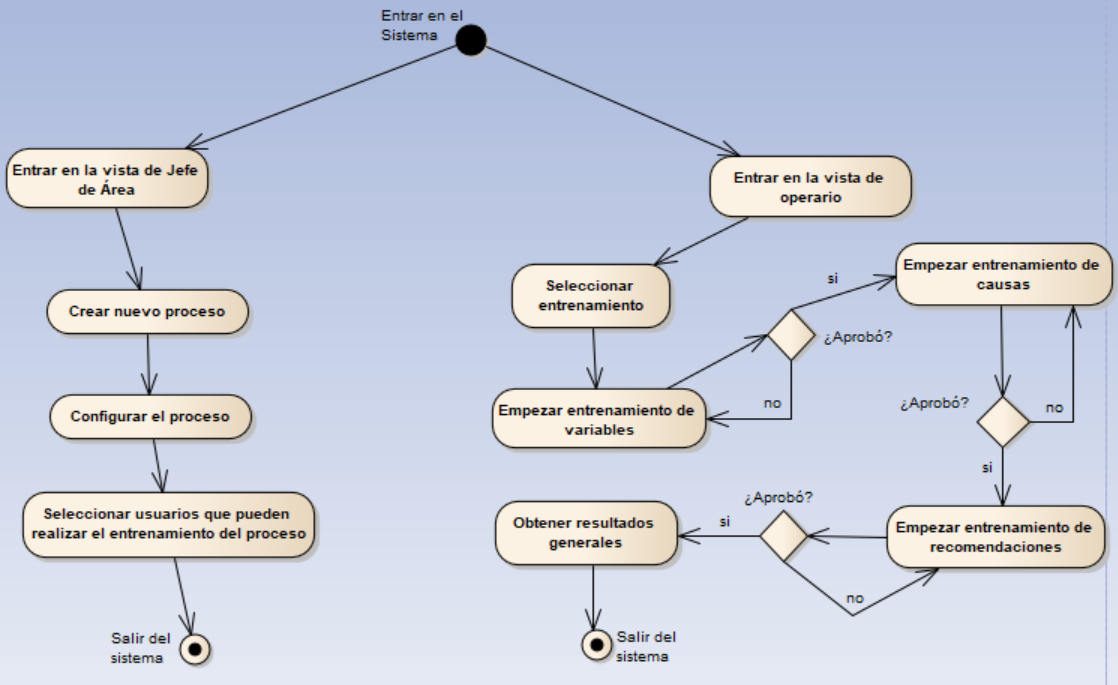
\includegraphics[width=0.7\linewidth]{imagen/actividades.png}
 \caption{Diagrama de actividades}
 \label{fig:actividades} 
\end{figure} 

%%%%%%%%%%%%%%%%%%%%%%%%%%%%%%%%%%%%%%%%%

\section{Captura de requisitos}
La extracción o captura de los requisitos en un sistema es una de las fases más críticas e importantes en el desarrollo de software. La fase de captura de requisitos tiene como objetivo descubrir y recoger todas las condiciones funcionales y no funcionales de una aplicación. Esta actividad de descubrimiento es una tarea más humana que técnica, ya que la mayor parte de las veces los usuarios no serán capaces de definir todas las condiciones \cite{Dave2022}. 

Para el desarrollo de este sistema se realizó un estudio de requisitos bastante extensivo. Se coordinó con los interesados y se acordó una lista de requerimientos funcionales y no funcionales.

\subsection{Requisitos funcionales}
Los requisitos funcionales son las declaraciones de los servicios que prestará el sistema. Cuando hablamos de las entradas, no necesariamente hablamos sólo de las de los usuarios, pueden ser interacciones con otros sistemas, respuestas automáticas, procesos predefinidos, entre otros. En algunos casos, los requisitos funcionales también establecen explícitamente lo que el sistema no debe hacer \cite{Dave2022}.

Los requisitos funcionales que posee esta solución ya incluyen los cambios presentados en el modelo de dominio. A las condiciones existentes en el sistema SECPROIT original se les agregó la configuración de los entrenamientos y la gestión de usuarios. Como resultado, los requisitos funcionales de este nuevo sistema son:

\begin{itemize}
\item \textbf{Cambiar contraseña personal}: es una acción que todos los usuarios pueden realizar.
\item \textbf{Iniciar sesión en el sistema}: es una acción que todos los usuarios pueden realizar.

\item \textbf{Gestionar usuarios}: es una actividad desarrollada solo por los administradores. Se basa en introducir, modificar y desactivar o activar los usuarios del sistema. También cuenta con una opción para restablecer la contraseña, en caso de que estos la hayan olvidado.
\item \textbf{Gestionar áreas}: es una actividad desarrollada solo por los administradores. Se basa en introducir, modificar y eliminar las áreas del sistema. Para poder eliminar un área laboral, esta debe estar vacía, es decir, que de ella no dependa ningún usuario.
\item \textbf{Ver acciones de los usuarios}: es una actividad desarrollada solo por los administradores. Permite observar, en una tabla, todas las actividades realizadas por los usuarios.

\item \textbf{Gestionar procesos}: es una actividad desarrollada solo por los jefes de área. Se basa en introducir, modificar y eliminar los procesos en un área laboral. Si se elimina un proceso, queda registro del mismo y los entrenamientos que se hayan realizado no se pierden.
\item \textbf{Configurar entrenamiento}: es una actividad desarrollada solo por los jefes de área. Consiste en asignar para cada proceso los estilos de pregunta que se pueden aplicar, la cantidad general de intentos, el tiempo máximo para realizar el entrenamiento y los usuarios que pueden evaluarse.
\item \textbf{Ver resultados de los operarios del área}: es una actividad desarrollada solo por los jefe de área. Permite observar, en una tabla, todos los resultados de los operarios que pertenezcan a esa área.

\item \textbf{Entrenamiento}: es una acción desarrollada solo por los operarios. Consiste en evaluarse sobre un proceso productivo. Se deben responder un conjunto de preguntas por etapas para luego obtener un resultado general que será registrado en el sistema.
\item \textbf{Ver resultados}: es una actividad desarrollada solo por los operarios. Permite observar, en una tabla, todos los resultados obtenidos en los entrenamientos.
\end{itemize}

\subsection{Requisitos No Funcionales}
Los requisitos no funcionales son condiciones que no se refieren directamente a las funciones específicas suministradas por un sistema (características de usuario), sino a las propiedades del mismo: rendimiento, seguridad, disponibilidad, entre otros. En palabras más sencillas, no hablan de lo que hace el sistema, sino de cómo lo hace. Alternativamente, definen restricciones del sistema tales como la capacidad de los dispositivos de entrada/salida y la representación de los datos utilizados en la interfaz del sistema \cite{Dave2022}.

En este caso, los requisitos no funcionales presentes en este nuevo sistema son los mismos del SECPROIT:

\begin{itemize}
\item \textbf{Usabilidad}: se debe garantizar un ambiente de trabajo simple e intuitivo, ya que la mayoría de los usuarios no poseen experiencias con sistemas informáticos
\item \textbf{Seguridad}: la información del sistema solo puede ser manipulada por usuarios autorizados (aquellos que posean usuario y contraseña)
\item \textbf{Confiabilidad}: se deben evitar los enlaces rotos, los ficheros de los procesos deben ser validados antes de utilizarlos y se debe garantizar la confidencialidad de la información
\item \textbf{Disponibilidad}: la aplicación de mecanismos de seguridad no debe constituir un retraso para el uso del sistema, el software siempre debe estar disponible, así como brindar su información actualizada
\item \textbf{Software}: se debe tener instalado el JDK versión 1.8 y la aplicación PostgreSQL versión 9.1 (mínimo) para el manejo de la base de datos
\item \textbf{Hardware}: se necesitan 64MB de memoria RAM, un microprocesador Pentium II a 450 MHz (mínimo), un disco duro con capacidad libre (mínima) de 4GB y un sistema operativo de entorno gráfico como Windows y Linux
\item \textbf{Portabilidad}: debe ser utilizado bajo sistemas operativos Windows o Linux, por lo que su desarrollo debe realizarse con un lenguaje y tecnologías capaces de brindar este soporte
\item \textbf{Restricciones en el diseño y la implementación}: debe desarrollarse sobre plataformas de software libre y código abierto y su lenguaje de programación debe ser Java, debido al uso de la herramienta \textsl{Drools}
\item \textbf{Políticos/Culturales}: debe encontrarse en idioma español
\end{itemize}

%%%%%%%%%%%%%%%%%%%%%%%%%%%%%%%%%%%%%%%%%